  %%%%%%%%%%%%%%%%%%%%%%%%%%%%%%%%%%%%%%% -*- coding: utf-8; mode: latex -*- %%
  %
%%%%%                     IMPLEMENTATION
 %%%
  %

\chapter{Implementation}

\label{ch:implemenation}

\begin{quotation}
"Keep it simple, stupid" K-I-S-S, is an acronym as a design principle noted by the U.S. Navy in 1960. The KISS principle states that most systems work best if they are kept simple rather than made complex; therefore simplicity should be a key goal in design and unnecessary complexity should be avoided.
{\small\it -- Kelly Johnson, aircraft engineer (1910 - 1990)}
\end{quotation}

  %%%%%%%%%%%%%%%%%%%%%%%%%%%%%%%%%%%%%%%%%%%%%%%%%%%%%%%%%%%%%%%%%%%%%%%%%%%%%

This chapter deals with all the topics related to the implementation of the solution that was proposed in Chapter 3. Important points are reviewed and will explained in more detail such as the the working tools, the QoD module and the process follow to develop and introduce the necessary changes made into the original HBase implementation before this action took place. The chapter is organized as follows. Firstly we give an overview of the itinerary followed in~\ref{roadmap}. Section~\ref{proposal} describes the architecture of the existing and proposed system very briefly. In Section~\ref{integration} the inner-workings of the main extensions made are outlined, namely modifications to existing classes in HBase and addition of new ones to the source code of the system. That is, the QoD module and some of its most important aspects. In addition to that, in part~\ref{grouping} we also explain how to group updates and what are the benefits of it. Later, in section~\ref{method} the methodology used to develop the solution is described. The final section~\ref{summary-implementation} summarizes the chapter and some of the most important points made.

 %%%%%%%%%%%%%%%%%%%%%%%%%%%%%%%%%%%%%%%%%%%%%%%%%%%%%%%%%%%%%%%%%%%%%%%%%%%%%
  %
%%%%%                        SECTION
 %%%
  %
\section{Roadmap}\label{roadmap}
In distributed scenarios, Facebook is currently using HBase to manage very large number of messages across data centers for their users, and not Cassandra~\cite{FacebookHBase} That is because of the simplicity of consistency model, as well as the ability of HBase to handle both a short set of volatile data and an ever-growing amount, that rarely gets accessed more than once. More specifically, in their architecture reports, a Key for each element is the userID as RowKey, word as Column and messageID as Version and finally the value like offset of word in message (Data is sorted as \emph{userId, word, messageID} ). That implicitly means that searching for the top messageIDs of an specific user and word is easily supported, and therefore queries run faster in the backend.

With eventual consistency, updates and insertions are propagated asynchronously between clusters so Zookeeper is used for storing their positions in log files that hold the next log entry to be shipped in Hbase. To ensure cyclic replication (master to master) and prevent from copying same data back to the source, a sink location with remote procedure calls invoked is already into place with HBase. Therefore if we can control the edits to be shipped, we can also decide what is replicated, when or in other words how often. Keeping that in mind, we leverage the internal mechanisms of VFC$^{3}$ to tune HBase consistency, without requiring intrusion to the data schema and avoiding middle-ware overhead.

For filtering purposes, with our new proposal and implementation, we will enable administrators of the clusters to create quality-of-data policies that can analyze fetched data by inspecting some given bounds or semantics, and then receiving them on the master server at the other end of the replication chain if a match occurs. The term "Tunable" or "Enhanced" \emph{eventual consistency} is sparingly used across the text to describe the model presented on inter-site replication scenarios of HBase. The goal is providing an adaptive consistency model and based on Service Level Objectives agreed or defined previously by users or clients. The idea can be somehow similar to the "pluggable replication framework" proposed within the HBase community we reference in this text.


  %%%%%%%%%%%%%%%%%%%%%%%%%%%%%%%%%%%%%%%%%%%%%%%%%%%%%%%%%%%%%%%%%%%%%%%%%%%%%
  %
%%%%%                        SECTION
 %%%
  %

\section{Extensions to the HBase internal mechanisms}\label{proposal}
The initial approach follows built-in properties of HBase in regards to HDFS. We use the WALEdit data structure of Hbase rather than reinventing the wheel. A WALEdit structure contains information about the incoming updates to the tables in the system and it is later saved in the form of HLog entry, in that write ahead log as it needs to be be committed to persistent storage later, HDFS.

In Hbase we modify its inner workings by populating and sorting a custom priority queue of items to be replicated until at a later stage a thread is triggered to pick up one at a time and then copy the relevant entries into another queue that will ship the rows to the remote location with the usual HBase mechanism.

%% Start by presenting our model, constraints, data containers, and how things work (are enforced / evaluated )
The QoD paradigm implemented allows for entries to be evaluated prior to replication based on one or several of the three parameters in a three-dimensional vector K ($\theta$, $\sigma$, $\nu$), corresponding to Time, Sequence, Value respectively in our case. Secondly, we take care of updates that collide with previous ones (same keys but different values). They can also be checked for number of pending updates or value difference from previously replicated updates, and then shipped or kept on the data structure accordingly. The time constraint can be always validated every X seconds, and the other two constraints are validated through Algorithm.~\ref{algo1}, whenever updates arrive. For the work presented here we use Sequence ($\sigma$) as the main vector-field bound (\texttt{HBaseQoD.enforce(containerId)}).

  %%%%%%%%%%%%%%%%%%%%%%%%%%%%%%%%%%%%%%%%%%%%%%%%%%%%%%%%%%%%%%%%%%%%%%%%%%%%%
  %
%%%%%                     SECTION
 %%%
  %

\section{How to integrate a Quality of Data (QoD) module into HBase}\label{integration}
To achieve that, it is necessary to modify HBase inner workings by creating, populating and sorting a custom priority queue of items to be replicated. At a later stage, those items will be picked up by a thread which triggers replication one at time or by grouping them into a single operation. In order to do that, we devised a first experiment with a vector-field data structure as described below in Listing~\ref{lst:vector-listing}.

\begin{lstlisting}[caption={K.java},label={lst:vector-listing}]

package org.apache.hadoop.hbase.replication.regionserver;

	public class K implements Comparable<K> {
	    private long time;
	    private int sequence;
	    private double value;

	    public K(long time, int sequence, double value) {
	        this.time = time;
	        this.sequence = sequence;
	        this.value = value;
	    }

	    public long getTime() {
	        return time;
	    }

	    public void setTime(long time) {
	        this.time = time;
	    }

	    public int getSequence() {
	        return sequence;
	    }

	    public void setSequence(int sequence) {
	        this.sequence = sequence;
	    }

	    public double getValue() {
	        return value;
	    }

	    public void setValue(double value) {
	        this.value = value;
	    }

	    public void incSequence() {
	        this.sequence++;
	    }

	    public void reset() {
	        this.sequence = 0;
	        this.value = -1;
	        this.time = -1;
	    }

	    @Override
	    public int compareTo(K o) {
	        if (o.sequence > 0 && sequence > o.sequence)
	            return 1;

	        return 0;
	    }

	    @Override
	    public String toString() {
	        return "K(" + time + ", " + sequence + ", " + value + ")";
	    }
	}

\end{lstlisting}


Regarding grouping of operations, we aim at finding a suitable way to enforce related updates in a single and timely replicated batch. This is possible, keeping in mind that individual updates using regular eventual consistency used in HBase can still arrive earlier, although not together and therefore causing bandwidth consumption more often.  into \emph{ReplicationSource.java} we have the following listing showing the main modifications in Listing~\ref{lst:filtering-listing}

\begin{lstlisting}[caption={ReplicationSource.java},label={lst:filtering-listing}]
        Entry[] filteredUpdates = filterEntriesToReplicate(Arrays.copyOf(entriesArray,currentNbEntries));
        
        //Print contents in cache 
        System.out.println(cache.toString());


                if(filteredUpdates.length > 0) {
                  try {
                      // Propagate changes now according to QoD constraints in filteredUpdates.

                      long now = System.currentTimeMillis();
                      System.out.println("*** Latest update sent at timestamp : " + now + " ***\n");
      
                      rrs.replicateLogEntries(Arrays.copyOf(filteredUpdates, filteredUpdates.length));
                      //getRS().replicateLogEntries(Arrays.copyOf(filteredUpdates, filteredUpdates.length));
                      } catch (IOException e) 
                      {
                              System.out.println("IOEXception caught while replicating: " + e.getStackTrace());
                      }
                }
\end{lstlisting}



%% Build up here on WAL, ReplicationSource, etc. Also architecture drawings.

%In order to provide bounded consistency guarantees with QoD, we add it to the inner workings of Hbase. There are existing command line tools as CopyTable in HBase where one can manually define what is going to be replayed to the log and this is useful for cases where new replicas need to be put up to date or in disaster recovery too. 

We focus the implementation efforts into the correctness of the list of items in memory (extending the original structure reflected for the updates to be shipped), which we can apply to our QoD model therefore directly in order to enforce desired consistency constraints. We do that by defining our bounded model over data which is indexed and queried by key (containerId), and can be enforced through time constraints (T), sequence (number of pending updates) and value ( percentage of changes). For the prototype just sequence. In other words \texttt{HBaseQoD.enforce(containerId)}.

% Keep building on it here. Talk about the WALPlayer and possibly how to replay messages but not only.
Every new update is checked for QoD and shipped for replication, or buffered as usual in HBase for replication, with the difference that using the QoD vector-field model one can immediate replicate updates at the moment of reaching a defined QoD condition. The QoD allows for entries to be evaluated by one or several of the three parameters as seen in vector field consistency \emph{K (time, sequence value)}~\cite{Santos:2007} Any new updates over previous ones (same data) can be also checked for number of pending updates or value difference from previously replicated update, and then shipped or kept on the data structure accordingly.

The original HBase architecture has built-in properties derived from the underlying HDFS layer. As part of it, the WALEdit data structure is used to store data temporarily before being replicated, useful to copy data between several HBase locations. The QoD algorithm (shown in Algorithm.~\ref{algo1}) uses that data structure, although we extend it to contain more meaningful information that help us in the management of the outgoing updates marked for replication.

% High-level algorithm we use to modify queued items for replication
\begin{algorithm*}
\caption{QoD high-level algorithm for filtering updates}
\label{algo1}
\begin{algorithmic}[1]
\REQUIRE $containerId$
\ENSURE $maxBound \neq 0$ and $controlBound \neq 0$
%\STATE $y \leftarrow 1$
\WHILE{$enforceQoD (containerId)$}
\IF{$getMaxK(containerId) = 0$}
\RETURN $true$
\ELSE[$getactualK(containerId)$]
\STATE $actualK(\sigma) \leftarrow actualK(\sigma)+1$
	\IF{$actualK(\sigma) \geq containerMaxK(\sigma)$}
	\STATE $actualK(\sigma) \leftarrow 0$
	\RETURN $true$
	\ELSE
	\RETURN $false$
	\ENDIF
\ENDIF
\ENDWHILE
\end{algorithmic}
\end{algorithm*}

  %%%%%%%%%%%%%%%%%%%%%%%%%%%%%%%%%%%%%%%%%%%%%%%%%%%%%%%%%%%%%%%%%%%%%%%%%%%%%
  %
%%%%%                         SECTION
 %%%
  %
\subsection{Operation Grouping}\label{grouping}
At the application level, it may be useful for HBase clients to enforce the same consistency level on groups of operations despite affected data containers having different QoD bounds associated. In other words, there may be specific situations where write operations need to be grouped so that they can be all handled at the same consistency level and propagated atomically to slave clusters. 

For example, publication of user statuses in social networks is usually handled at eventual consistency, but if they refer to new friends being added (e.g., an update to the data container holding the friends of a user), they should they should be handled at a stronger consistency level to ensure they are atomically visible along with the list of friends of the user in respect to the semantics we describe here.

In order to not violate QoD bounds and maintain consistency guarantees, all data containers of operations being grouped must be propagated either immediately after the block execution, or when any of the QoD bounds associated to the operations has been reached. When a block is triggered for replication, all respective QoD bounds are naturally reset. 

To enable this behavior we propose extending the HBase client libraries to provide atomically consistent blocks.
Namely, adding two new methods to HTable class in order to delimit the consistency blocks: \textit{startConsistentBlock} and \textit{endConsistentBlock}. Each block, through the method \textit{startConsistentBlock}, can be parameterized with one of the two options: i) \textit{IMMEDIATE}, which enforces stronger consistency for the whole block of operations within it; and ii) \textit{ANY}, which replicates a whole block as soon as any QoD vector field bound, associated with an operation inside the block is reached.

Next, in Listing~\ref{lst:group-listing} we provide an illustrative simple example of a social network where three containers with different consistency levels are modified. Note that we are not aiming at full transactional support, as it would be possible to change the same data containers modified by a set of grouped operations, at the same time, from other operations individually.

\begin{lstlisting}[language={java}, caption={Operation grouping},label={lst:group-listing}]
htable.startConsistentBlock(ConsistencyType.IMMEDIATE)
Put put1 = new Put(Bytes.toBytes("row1"));
put1.add(Bytes.toBytes("SocialNetTable"),Bytes.toBytes("status"), Bytes.toBytes("friend 12345 added"));

Put put2 = new Put(Bytes.toBytes("row2"));
put2.add(Bytes.toBytes("SocialNetTable"), Bytes.toBytes("friends"), Bytes.toBytes("12345"));

Put put3 = new Put(Bytes.toBytes("row3"));
put3.add(Bytes.toBytes("SocialNetTable"), Bytes.toBytes("wall"), Bytes.toBytes("12345 is now a friend"));

htable.put(put1);
htable.put(put2);
htable.put(put3);

htable.endConsistentBlock();
\end{lstlisting}

\subsection{Proposed scenario}
One of the key factors for having operations grouping working together with HBase-QoD is the depicted in Figure~\ref{fig-qod-grouping}. We can see that the operations that are grouped need to communicate over the network less often to other clusters, while arriving earlier in some cases than updates shipping as if several individual operations from location Cluster A were performed. This is due to the ability of HBase-QoD to deliver demanded updates in a consistent timely-fashion rather than on a per request arrival basis, which means possibly delaying the replication process by a fraction of the amount of communication that can be saved instead using the mentioned technique.

\begin{figure}[t]
\centering
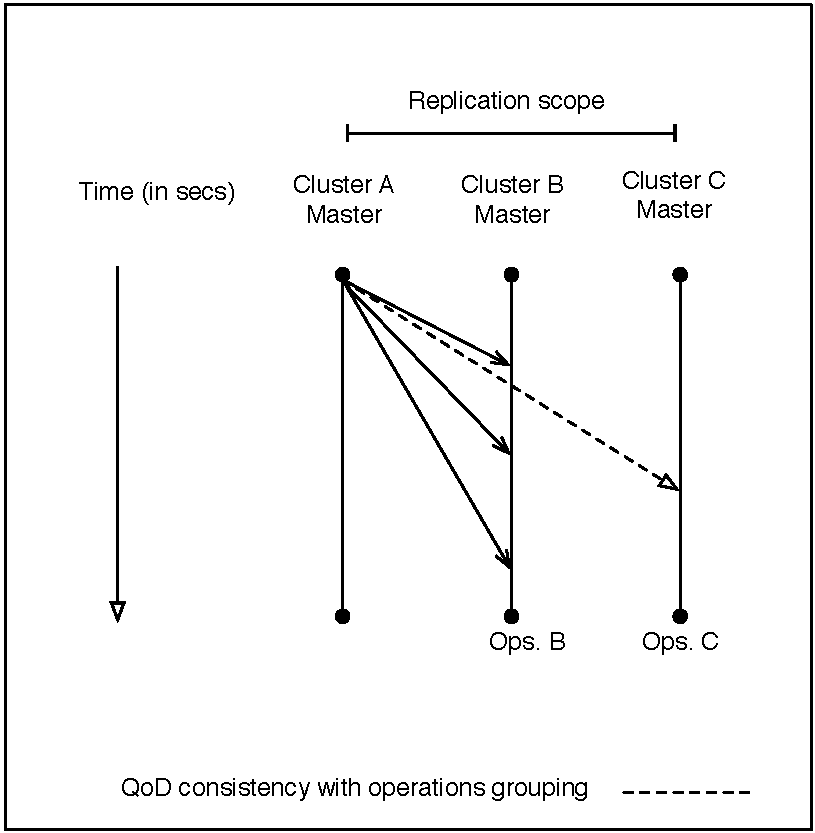
\includegraphics[scale=0.6]{figs/operation-grouping.pdf}
\caption{Resulting scenario of grouping operations in a time-lined based diagram using HBase-QoD versus a regular HBase deployment at Cluster B}
\label{fig-qod-grouping}
\end{figure}

Another experiment that has been conclusive in terms of grouping of operations is the comparison between different QoD levels, in the case of values for vector field K (-, $\sigma$, -). Setting the operation grouping for a small number of updates still shows that a timestamp in the receiving server is the same for every item in the group. The following set of operations is reflect in Figures~\ref{fig-shipping-grouping} and ~\ref{fig-receiving-grouping}. The same principle can be applied and has been demonstrated to work in the same fashion for different sets of containers.

%(table_name::columnFamily).

\begin{figure}[b]
\centering
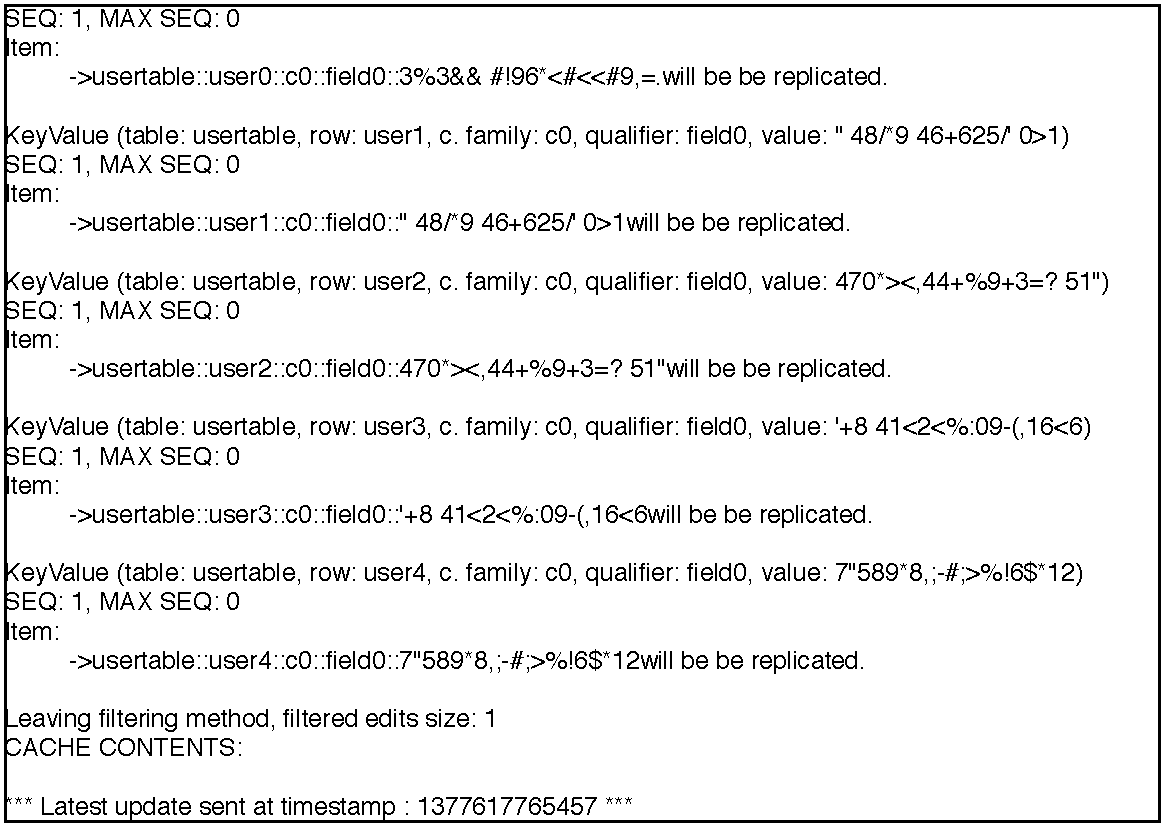
\includegraphics[scale=0.6]{figs/ginja2-grouping-send.pdf}
\caption{Sending from ginja-a2 to ginja-a1}
\label{fig-shipping-grouping}
\end{figure}

In the following Figure~\ref{fig-receiving-grouping}, we observe how the timestamp for each of the items replicated from the grouped operation have the same timestamp (\textbf{1377617765557}) at the receiving side on ginja-a1. That ensures they have arrived at the same time, and actually we verify the correctness of the experiment by leveraging internal HBase mechanisms that are currently being already used to list statistics of the age of updates sent and/or receive. At the sending side on the other hand, each update is grouped until finally they are all due to be replicated as a whole and therefore printing the timestamp only in order to comply with the reality.

\begin{figure}[t]
\centering
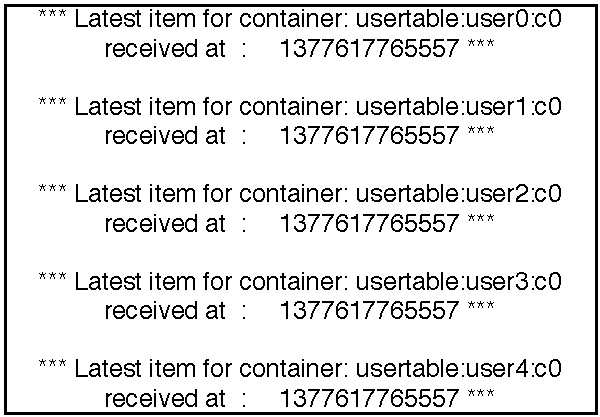
\includegraphics[scale=.6]{figs/ginja1-grouping-receive.pdf}
\caption{Receiving from ginja-a2 in ginja-a1}
\label{fig-receiving-grouping}
\end{figure}
 


  %
 %%%
%%%%%                           SECTION
  %
  %%%%%%%%%%%%%%%%%%%%%%%%%%%%%%%%%%%%%%%%%%%%%%%%%%%%%%%%%%%%%%%%%%%%%%%%%%%%%


\section{Implementation remarks}\label{summary-implementation}
The main problems and proposed solutions have been introduced in this section. In the following chapter we will evaluate our proposal and show some insights about the correlation between expected and actual results.

%%% Local Variables: 
%%% mode: latex
%%% TeX-master: "tese"
%%% End: 
